# version 0.9.1
\begin{center}
\Huge{\pack } \\
\Large{An \R~package to visualize outputs from the data base \BDfull~(\BD)}

~\\

version \versionnumber \\

~\\
\today

~\\~\\

Pierre Rivi\`ere\textsuperscript{1,2} \hspace{1cm} Yannick de Oliveira\textsuperscript{3} \\
~\\~\\ 
\end{center}


\noindent\textsuperscript{1} R\'eseau Semences Paysannes, 3 avenue de la gare, F-47190 Aiguillon, France \\ 
\textsuperscript{2} INRA, UMR 0320, Génétique Quantitative et Evolution, DEAP team, Ferme du Moulon F-91190 Gif sur Yvette, France \\
\textsuperscript{3} INRA, UMR 0320, Génétique Quantitative et Evolution, ABI team, Ferme du Moulon F-91190 Gif sur Yvette, France \\
\textbf{Contact:} \href{mailto:pierre@semencespaysannes.org}{pierre@semencespaysannes.org} \\
\textbf{Contributions:} 
P. Rivière worte the \texttt{R} functions and the vignette,
Y. de Oliveira wrote the \texttt{SQL} queries.

\vfill

\begin{center}
Copyright Réseau Semences Paysannes and Institut National de la Recherche Agronomique \\
\href{http://creativecommons.org/licenses/by-nc-sa/4.0/}{Licence creative commons BY-NC-SA 4.0} \\
\vspace{.25cm}
\href{http://creativecommons.org/licenses/by-nc-sa/4.0/}{
\includegraphics[width=.15\textwidth]{cc-by-nc-sa}}
\end{center}

\vfill

\begin{wrapfigure}{l}{.15\textwidth}
\begin{center} \vspace{-20pt}
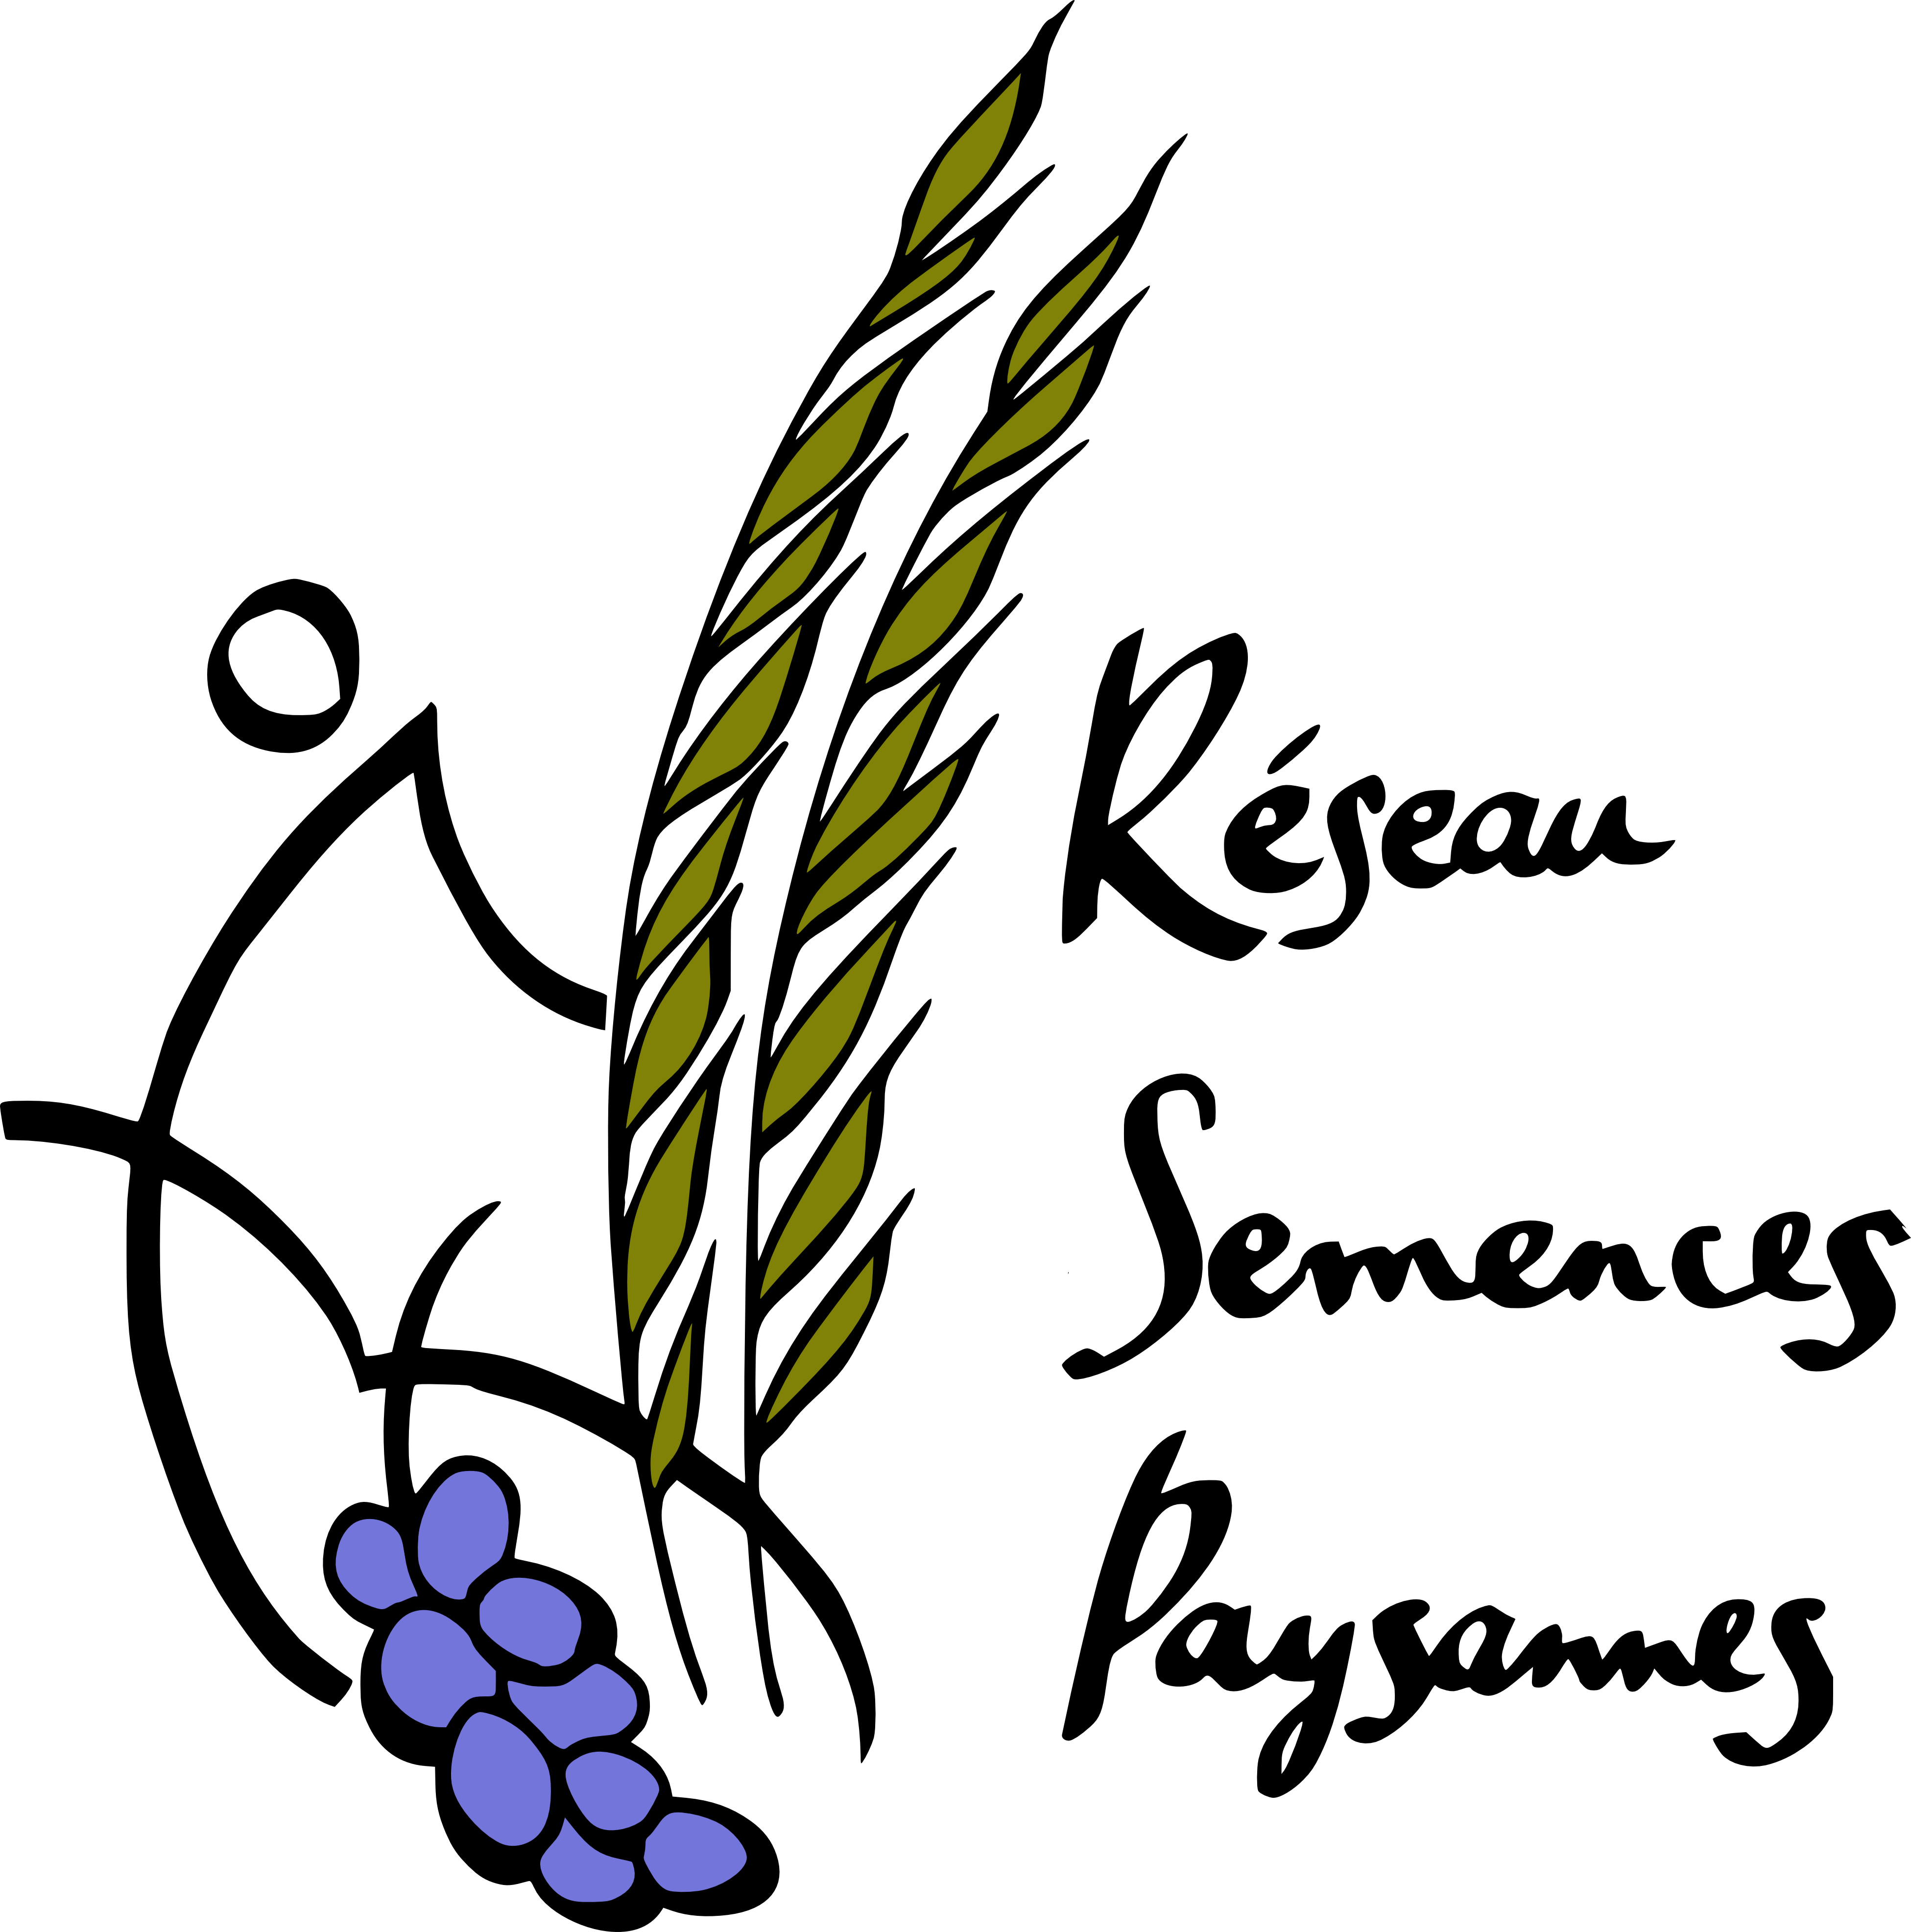
\includegraphics[width=.15\textwidth]{Logo-RSP}
\end{center} \vspace{-20pt}
\end{wrapfigure}
\noindent
Le Réseau Semences Paysannes (the French Farmers' Seeds Network (RSP)), created in 2003, brings together a great diversity of collectives and people who preserve farmers' seeds in fields, orchards, vineyards and gardens. They are involved in supporting the consolidation of local initiatives to maintain and renew cultivated biodiversity through Community Seeds Systems. Over 80 organizations have come together to promote and develop farmers' seeds, and to protect farmers' rights over their seeds. \\
\url{www.semencespaysannes.org} (in french).


\vfill

\begin{wrapfigure}{l}{.15\textwidth}
\begin{center} \vspace{-20pt}
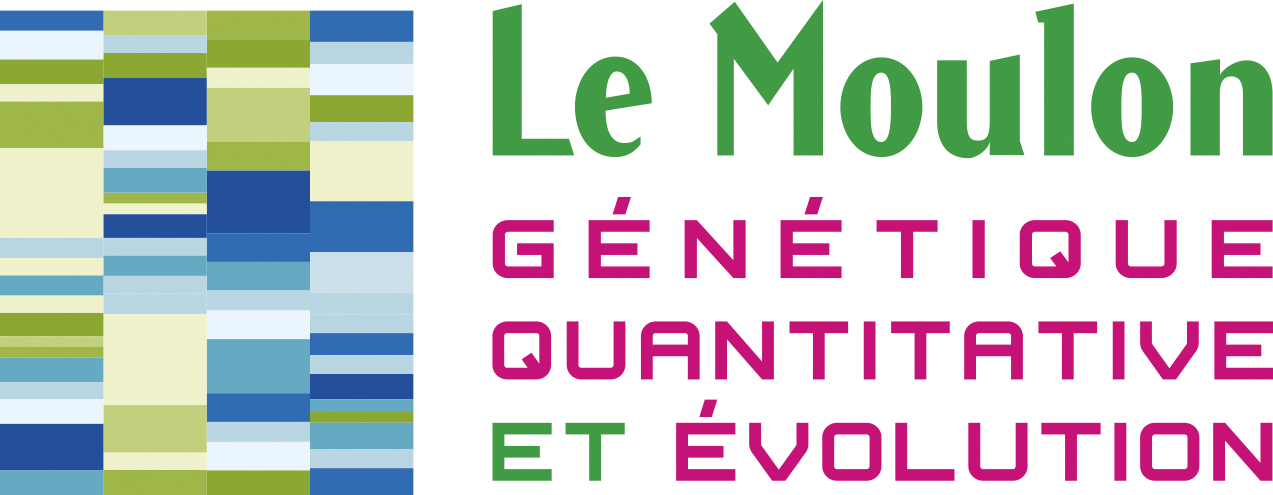
\includegraphics[width=.15\textwidth]{Logo-UMRGV}
\end{center} \vspace{-20pt}
\end{wrapfigure}
\noindent
The Diversity, Evolution and Adaptation of Populations (DEAP) team led by Isabelle Goldringer is part of INRA UMR 0320 Quantitative Genetic and Evolution.
Its work is based on the analysis of the genetic and evolutionary mechanisms underlying evolution and adaptation of crop populations.
DEAP develops strategies for on farm management of crop genetic diversity and
for plant breeding (evolutionary and/or participatory) adated to organic and low input agriculture.
Assessing the benefits of in-field genetic diversity (variety mixtures, populations) and designing
/ breeding optimized mixtures adapted to local conditions are also key research objectives.\\
\url{http://moulon.inra.fr/index.php/en/team/deap} \\
\noindent
The bioinformatics and informatics facility (ABI, Atelier Bioinformatique et Informatique) provides bioinformatics expertise and IT support. The staff includes 6 experts in system administration, software development or bio-analysis, and develops databases and softwares for proteomics, genetics and genomics. ABI offers hardware resources, scientific programming and consulting for DNA, RNA and protein sequence analysis up to genome-wide scale. ABI works in tight collaboration with the Bioinformatics facilities of University Paris-Sud and INRA, and contributes to the future French Bioinformatics Institute. \\
\url{http://moulon.inra.fr/index.php/en/tranverse-team} \\


\vfill




\newpage

\tableofcontents

\vfill

\begin{center}
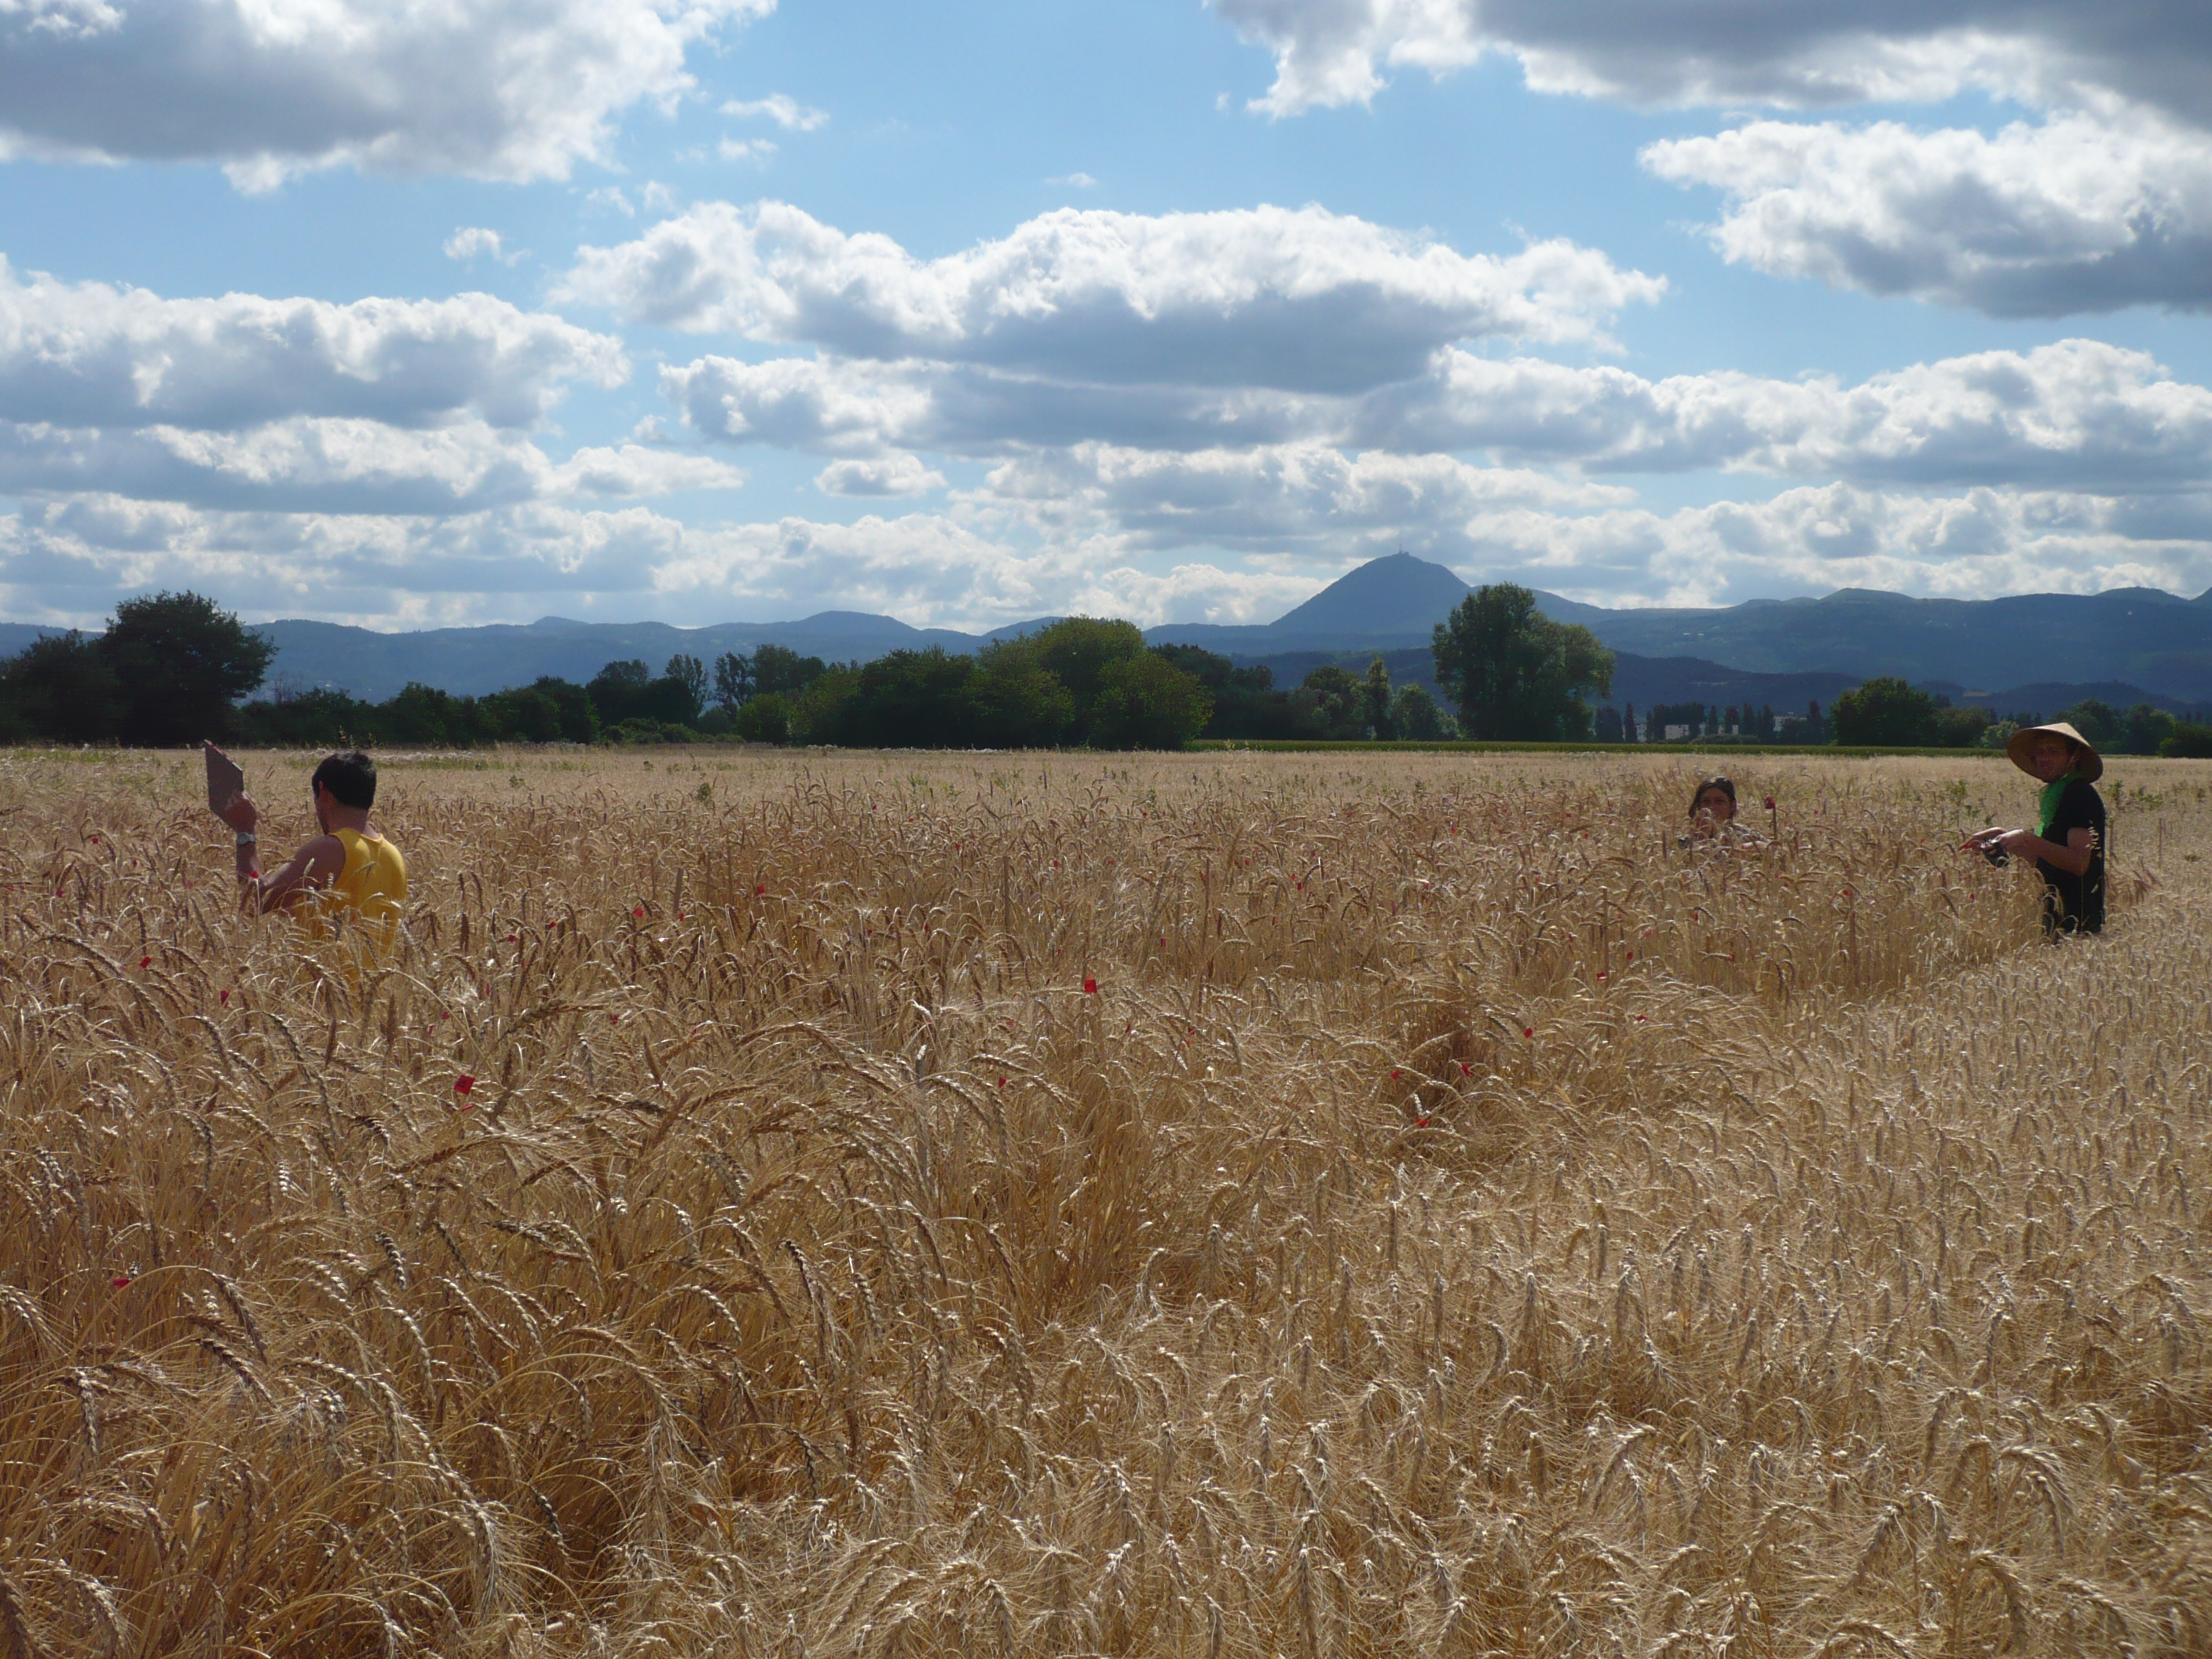
\includegraphics[width=.8\textwidth]{wheat} \\
Wheat trials on farm within our participatory plant breeding programme, summer 2012, Auvergne, France. \\
CC-BY-NC-SA. Pierre Rivière.
\end{center}

\newpage
\pagestyle{plain}
